\documentclass{beamer}
\usepackage{beamerthemeshadow}
\usepackage{graphicx}
\usepackage{color}
\usepackage[utf8]{inputenc}
\usepackage{hyperref}
\usepackage[flushleft]{threeparttable}
\definecolor{beamer@blue}{rgb}{0.85,0.1,0.1}
\setbeamercolor{structure}{fg=beamer@blue}
\usetheme{Berkeley}

\def\d{{\fontencoding{T1}\selectfont\dj}}
\def\D{{\fontencoding{T1}\selectfont\DJ}}

\begin{document}
\title{Džonatan Bouen}

\author{\flushleft Vladimir Jovanović \and\\ Andrea Mefailovski Stanojević \and\\ Marija Papović \and\\ Katarina Grbović }
\institute{\flushright Matematički fakultet\\Univerzitet u Beogradu}
\date{
	\footnotesize{Beograd, 2019.}	
}

\begin{frame}
	\thispagestyle{empty}
	\titlepage
\end{frame}

\addtocounter{framenumber}{-1}

\begin{frame}{Džonatan Piter Bouen}
    \begin{center} 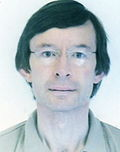
\includegraphics[scale=3]{Jonathan_Bowen_photograph.jpg} \end{center}
    \begin{itemize}
        \item Britanski stručnjak za računare
        \item Predstavnik i osnivač "Museophile Limited" kompanije
        \item Profesor emeritus na \textit{London South Bank} univerzitetu
    \end{itemize}
\end{frame}

\begin{frame}
	\frametitle{Obrazovanje}
	\begin{itemize}
		\item Ro{\d}en je u Okfsordu 1956.
		\item Školovao se u "Dragon School" (Oksford) i u školi u Brajanstonu 
		\item Maturirao je na Univerzitetskom koledžu u Oksfordu, gde je stekao zvanje magistra inženjerskih nauka
		\item[]
		\item[] \begin{center} 
\includegraphics[scale=0.25]{University_College_Oxford_Coat_Of_Arms.png} \hspace{25} 
\includegraphics[scale=0.3]{Dragon_Coat_Of_Arms.png} \end{center}
	\end{itemize}
\end{frame}

\begin{frame}[fragile]\frametitle{Literatura}
	\begin{itemize}
		\item Zasnovano na:\\
		wiki stranica
	\end{itemize}
\end{frame}

\begin{frame}{Karijera}
    \begin{center} 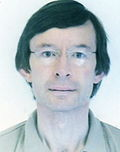
\includegraphics[scale=3]{Jonathan_Bowen_photograph.jpg} \end{center}
    \begin{itemize}
        \item Radio na koledžu u Londonu
        \item Radio u kompjuterskoj laboratoriji univerziteta u Oksfordu
        \item Profesor na \textit{London South Bank} univerzitetu
    \end{itemize}
\end{frame}

\begin{frame}{Karijera}
    \begin{center} 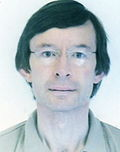
\includegraphics[scale=3]{Jonathan_Bowen_photograph.jpg} \end{center}
    \begin{itemize}
        \item Svoj rad zasnivao na formalnim metodama i z-notacijama
        \item Predstavnik britanskog kompjuterskog društva
        \item Pomoćnik urednika za više novina o oblasti softverskog inženjerstva
	\begin{center} 
\includegraphics[scale=3]{BCS-FACS_logo.jpg} \end{center}
    \end{itemize}
\end{frame}

\end{document}
